\documentclass{beamer}
\mode<presentation>
\usepackage{amsmath}
\usepackage{amssymb}
\usepackage{bm}
\usepackage{adjustbox}
\usepackage{subcaption}
\usepackage{enumerate}
\usepackage{multicol}
\usepackage{mathtools}
\usepackage{listings}
\usepackage{url}
\def\UrlBreaks{\do\/\do-}
\usetheme{Boadilla}
\usecolortheme{lily}
\setbeamertemplate{footline}
{
  \leavevmode%
  \hbox{%
  \begin{beamercolorbox}[wd=\paperwidth,ht=2.25ex,dp=1ex,right]{author in head/foot}%
    \insertframenumber{} / \inserttotalframenumber\hspace*{2ex} 
  \end{beamercolorbox}}%
  \vskip0pt%
}
\setbeamertemplate{navigation symbols}{}

\providecommand{\nCr}[2]{\,^{#1}C_{#2}}
\providecommand{\nPr}[2]{\,^{#1}P_{#2}}
\providecommand{\mbf}{\mathbf}
\providecommand{\pr}[1]{\ensuremath{\Pr\left(#1\right)}}
\providecommand{\qfunc}[1]{\ensuremath{Q\left(#1\right)}}
\providecommand{\sbrak}[1]{\ensuremath{{}\left[#1\right]}}
\providecommand{\lsbrak}[1]{\ensuremath{{}\left[#1\right.}}
\providecommand{\rsbrak}[1]{\ensuremath{\left.#1\right]}}
\providecommand{\brak}[1]{\ensuremath{\left(#1\right)}}
\providecommand{\lbrak}[1]{\ensuremath{\left(#1\right.}}
\providecommand{\rbrak}[1]{\ensuremath{\left.#1\right)}}
\providecommand{\cbrak}[1]{\ensuremath{\left\{#1\right\}}}
\providecommand{\lcbrak}[1]{\ensuremath{\left\{#1\right.}}
\providecommand{\rcbrak}[1]{\ensuremath{\left.#1\right\}}}
\providecommand{\rank}{\text{rank}}
\theoremstyle{remark}
\newtheorem{rem}{Remark}
\newcommand{\sgn}{\mathop{\mathrm{sgn}}}
\providecommand{\abs}[1]{\ensuremath{\left\vert #1 \right\vert}}
\providecommand{\res}[1]{\Res\displaylimits_{#1}} 
\providecommand{\norm}[1]{\lVert#1\rVert}
\providecommand{\mtx}[1]{\mathbf{#1}}
\providecommand{\mean}[1]{\overline{#1}}
\providecommand{\fourier}{\overset{\mathcal{F}}{ \rightleftharpoons}}
\providecommand{\system}{\overset{\mathcal{H}}{ \longleftrightarrow}}
\providecommand{\dec}[2]{\ensuremath{\overset{#1}{\underset{#2}{\gtrless}}}}

% this \vec is already defined in your file:
\renewcommand{\vec}[1]{\begin{pmatrix}#1\end{pmatrix}}

\newenvironment{amatrix}[1]{%
  \left(\begin{array}{@{}*{#1}{c}|c@{}}
}{%
  \end{array}\right)
}

\lstset{
frame=single, 
breaklines=true,
columns=fullflexible
}
\usepackage{listings}
\lstset{
  language=Python,
  basicstyle=\ttfamily\small,
  numbers=left,
  numberstyle=\tiny,
  breaklines=true,
  frame=single
}

\title{Matgeo-4.8.15}
\author{AI25BTECH11019-Menavath Sai Sanjana}

\date{}

\begin{document}
  
\begin{frame}  
\titlepage  
\end{frame}  
   

\begin{frame}  
\frametitle{Question}  
A line $l$ passes through point $(-1,3,-2)$ and is perpendicular to both the lines  
$\frac{x-1}{1} = \frac{y-1}{2} = \frac{z+1}{3}$ and  
$\frac{x+2}{-3} = \frac{y}{2} = \frac{z}{5}$. Find the vector equation of the line $l$ and its distance from the origin.  
\end{frame}  

\begin{frame}  
\frametitle{Solution } 

Let the direction vector of the required line be  
$
\vec{d} = \vec{a\\b\\c}.
$

Since the line is perpendicular to the two given lines, the direction vector satisfies
\begin{align}  
\vec{d}_1^\top \vec{d} &= 0 \quad \Rightarrow \quad 1\cdot a + 2\cdot b + 3\cdot c = 0,\\  
\vec{d}_2^\top \vec{d} &= 0 \quad \Rightarrow \quad -3\cdot a + 2\cdot b + 5\cdot c = 0.
\end{align}  


Solve the system:  
\begin{align}  
8b + 14c &= 0 \;\;\Rightarrow\;\; b = -\frac{7}{4}c,\\  
a + 2b + 3c &= 0 \;\;\Rightarrow\;\; a = \frac{1}{2}c.
\end{align}  
\end{frame}

\begin{frame}
\frametitle{Solution}
Choosing $c=4$ to get integer values:  
\begin{align}  
\vec{d} = \vec{2\\-7\\4}.
\end{align}  

Vector equation of the line through $P=(-1,3,-2)$:  
\begin{align}  
\vec{r} = \vec{-1\\3\\-2} + t\,\vec{2\\-7\\4}, \quad t \in \mathbb{R}.
\end{align}  

\end{frame}

\begin{frame}
\frametitle{Solution}
Distance from origin:  

\begin{align}  
t &= -\frac{\vec{P}\cdot\vec{d}}{\vec{d}\cdot\vec{d}} 
= -\frac{(-1)(2) + 3(-7) + (-2)(4)}{2^2 + (-7)^2 + 4^2} 
= \frac{31}{69},\\  
\vec{Q} &= \vec{P} + t\vec{d} = \vec{-\frac{7}{69}\\\\ -\frac{10}{69}\\\\ -\frac{14}{69}},\\  
D &= \|\vec{Q}\| = \sqrt{\frac{345}{69^2}} = \sqrt{\frac{5}{69}}.
\end{align}  

\end{frame}  

\begin{frame}  
\frametitle{Conclusion}  
\noindent\textbf{Conclusion:}  

The required line is  
$
\vec{r} = \vec{-1\\3\\-2} + t\,\vec{2\\-7\\4}, \quad t \in \mathbb{R},
$  
and its distance from the origin is  
$
D = \sqrt{\frac{5}{69}}.
$ 
\end{frame}


\begin{frame}
\frametitle{Graphical Representation}

\begin{figure}[ht!]
    \centering
    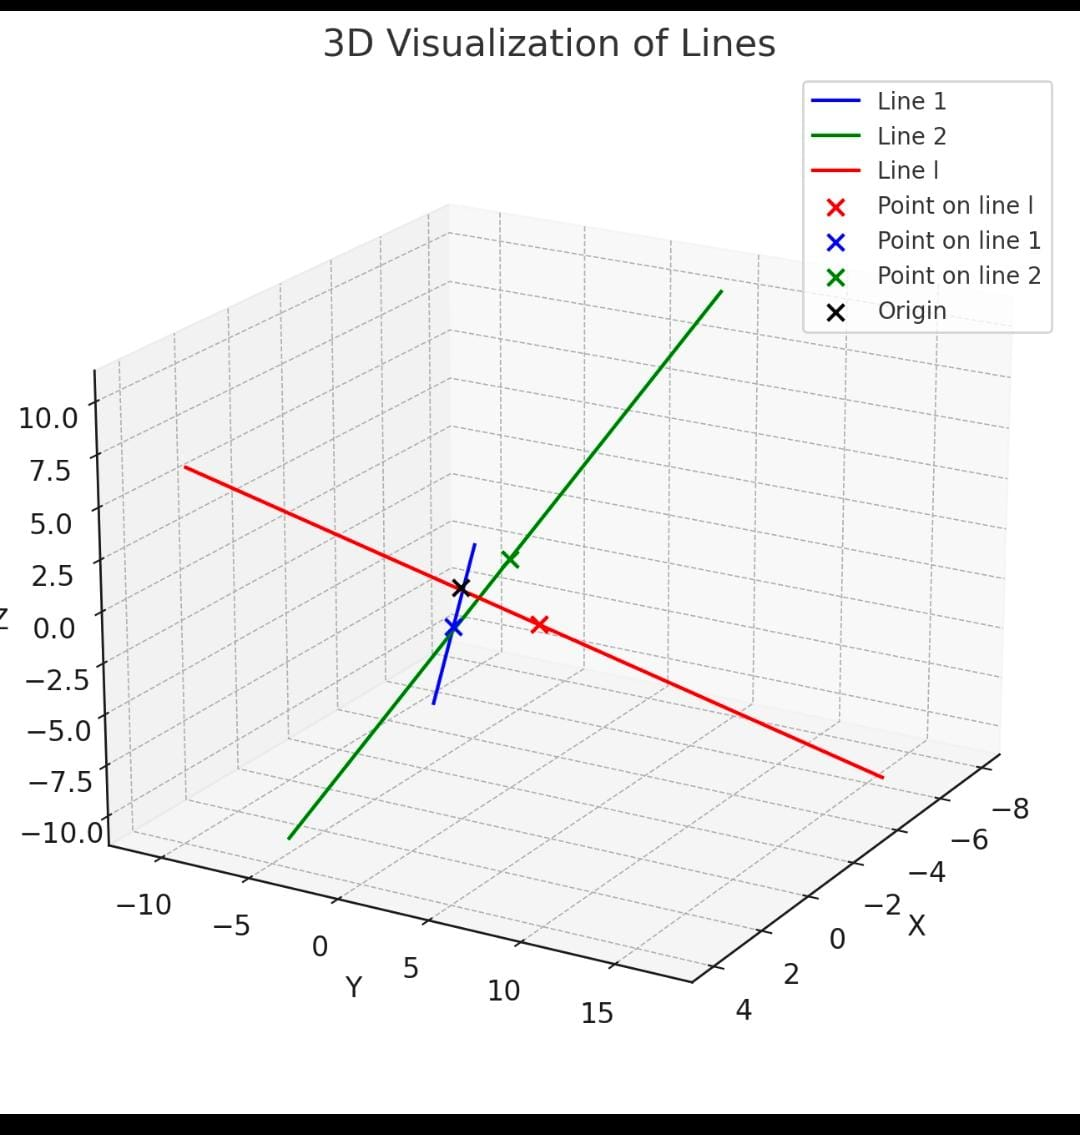
\includegraphics[width=0.65\textwidth]{matgeo-4.8.15.jpeg}
    \caption{}
    \label{fig:triangle5cm}
\end{figure}
\end{frame}

\end{document}
